\chapter{字符串管理}

任何程序都需要管理字符串。管理就像分配、搜索、连接、扩展、收缩等等。

字符串需要许多操作。 尽管C标准库为这一目标提供了许多功能,但C经典字符串,即\code{char *}(或\code{char []})在PHP这样的强程序中按原样使用通常有点弱。

因此,PHP在C字符串之上设计了一个层:\keyword{zend\_strings}。另外还存在另一个API,它实现了C经典字符串或\keyword{zend\_strings}常见的字符串操作: \keyword{smart\_str} API。

\section{字符串管理:zend\_string}

它增加了内存管理功能,以便相同字符串可以在多个地方共享,而不需要复制它。另外一些字符串被“扣押”,即它们被“持久”分配并由内存管理器专门管理,因此它们不会在多个请求中被销毁。 这些内存稍后将从\href{http://www.phpinternalsbook.com/php7/memory_management/zend_memory_manager.html}{Zend内存管理器}获得永久分配。

\subsection{结构和访问宏}

下面是\keyword{zend\_string}结构:

\begin{lstlisting}[language=c]
struct _zend_string {
        zend_refcounted_h gc;           /*gc信息*/
        zend_ulong        h;            /* hash value */
        size_t            len;          /*字符串长度*/
        char              val[1];       /*字符串起始地址*/
};
\end{lstlisting}

如您所见,该结构嵌入了\code{zend\_refcounted\_h}头。这样做是为了内存管理和引用。由于字符串很可能用作哈希表查询的键,所以它将其哈希值嵌入到\keyword{h}字段中。这是一个无符号long \code{zend\_ulong}。
此数字仅在需要对\code{zend\_string}进行哈希处理时使用,尤其是与\href{http://www.phpinternalsbook.com/php7/internal_types/hashtables.html}{HashTables zend\_array}一起使用时; 这很可能。


如您所知,可以通过\keyword{len}字段知道字符串的长度,用来支持“二进制字符串”。二进制字符串是嵌入一个或多个\keyword{NUL}字符(\textbackslash{}0)的字符串。当传递给libc函数时,这些字符串将被截断,否则它们的长度将无法正确计算。所以在\keyword{zend\_string}中,字符串的长度总是已知的。请注意,计算ASCII字符(字节)数量的长度,不计算结尾的\keyword{NUL},但是计算可能在中间的NULs。例如,字符串“foo”在\keyword{zend\_string}中存储为“foo\textbackslash{}0”,其长度为3。此外,字符串“foo\textbackslash{}0bar”将存储为“foo\textbackslash{}0bar\textbackslash{}0”,长度将为7。

最后,字符存储在\code{char [1]}字段中。这不是一个\code{char *},而是一个\code{char[1]}。为什么?这是一种名为“C struct hack”的内存优化。(你可以搜索一下这些术语)。基本上,它允许引擎为\code{zend\_string}结构和要存储的字符分配空间,作为一个单独的C指针。这优化了内存访问,因为内存将是一个连续分配的块,而不是内存中稀疏的两个块
(一个用于\code{zend\_string *},一个用于存储到其中的\code{char *})。

struct hack一定要记住,因为内存布局看起来像C字符位于C \code{zend\_string}结构的末尾,在使用C调试器(或在调试字符串时)时可能会感觉到/看到。这个hack完全由你在操作\code{zend\_string}结构时使用的API管理。

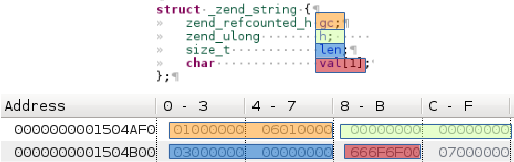
\includegraphics{images/zend_string_memory_layout.png} 

\subsection{使用\code{zend\_string} API}

\subsubsection{简单实例}

与\keyword{Zvals}一样,您不要手工操作\code{zend\_string}内部字段,而是始终要使用宏。还有一些宏可以触发字符串上的操作。这些不是函数,而是宏,都存储在所需的\href{https://github.com/php/php-src/blob/PHP-7.0/Zend/zend_string.h}{Zend/zend\_string.h }头:

\begin{lstlisting}[language=c]
zend_string *str;

str = zend_string_init("foo", strlen("foo"), 0);
php_printf("This is my string: %s\n", ZSTR_VAL(str));
php_printf("It is %zd char long\n", ZSTR_LEN(str));

zend_string_release(str);
\end{lstlisting}

上面的简单示例展示了基本的字符串管理。

\code{zend\_string\_init()}函数(它实际上是宏,但是让我们传入这些细节)应当传入完整\code{char *}型C字符串及其长度。最后一个参数(类型为int)值应该是0或1。如果传0,则要求引擎使用Zend内存管理器使用请求绑定堆分配。这种分配将在当前请求结束时销毁。如果您不这样做,在调试构建时,引擎将会对您刚刚创建的发出内存泄漏的警告。如果传1,您将请求我们所说的“持久”分配,即引擎将调用传统的C \code{malloc()}方法,并且不会以任何方式跟踪内存分配。

\alertinfo{如果您想了解有关内存管理的更多信息,可以阅读\href{http://www.phpinternalsbook.com/php7/memory_management.html}{专门章节}。}

然后,我们输出字符串。 我们使用\code{ZSTR\_VAL()}宏访问字符数组。\code{ZSTR\_LEN()}获取长度信息。 \code{zend\_string}相关的宏都以\code{ZSTR\_**()}开头,请注意这与\code{Z\_STR**()}宏不同。

\alertinfo{长度使用\code{size\_t}类型存储。因此为了输出它\code{printf()}需要使用"\%zd"。您应该始终使用正确的\code{printf()}格式。如果不这样做可能会导致应用程序崩溃或产生安全问题。有关printf()格式的精彩回忆,请访问\href{http://www.cplusplus.com/reference/cstdio/printf/}{此链接}}

最后,我们使用\code{zend\_string\_release()}释放字符串。这个"释放"是强制性的。这是关于内存管理的。“释放”是一个简单的操作:减少字符串的引用计数器,如果它变为0,API将为你释放字符串。如果忘记释放字符串,很可能会造成内存泄漏。

\alertinfo{您必须始终考虑C语言中的内存管理。如果您分配内存-无论是直接使用\code{malloc()},还是使用API来完成,你必须在某个时刻进行\code{free()}。如果不这样做会造成内存泄露并会变成没有人能够安全使用的设计糟糕的程序}

\subsubsection{使用hash}

如果需要访问hash值,请使用\code{ZSTR\_H()}。但是,创建\code{zend\_string}时不会自动计算哈希值。但是当使用HashTable API操作字符串时,它将会完成计算。如果你想强制立即计算hash值,可以使用\code{ZSTR\_HASH()}或者\code{zend\_string\_hash\_val()}。一旦计算出hash值,它将会被保存并且不会再次被计算。如果处于某种原因,您需要重新计算它 - 例如:因为你更改了字符串的值 - 使用\code{zend\_string\_forget\_hash\_val()}:



\begin{lstlisting}[language=c]
        zend_string *str;

        str = zend_string_init("foo", strlen("foo"), 0);
        php_printf("This is my string: %s\n", ZSTR_VAL(str));
        php_printf("It is %zd char long\n", ZSTR_LEN(str));
        
        zend_string_hash_val(str);
        php_printf("The string hash is %lu\n", ZSTR_H(str));
        
        zend_string_forget_hash_val(str);
        php_printf("The string hash is now cleared back to 0!");
        
        zend_string_release(str);
\end{lstlisting}


\subsubsection{字符串复制及内存管理}



